\section{Hadoop Security}
\label{security}
In this section, we discuss the security modules of Hadoop and the according security vulnerabilities: 1) arbitrary code execution; 2) malicious user impersonation; and 3) compromised nodes.
\subsection{Arbitrary code execution}
Arbitrary code execution occurs because Hadoop executes the code of the user-submitted jobs without inspection. It is common in Hadoop 1.x because MapReduce jobs submitted by malicious users could be executed with permissions of the TaskTracker while the TaskTracker is an independent Java process.

Since it is difficult to inspect MapReduce source code, the best way is to restraint the damages of arbitrary code execution. YARN container could isolate tasks and limits task privilege. It has three implementations of container executor: 1) Default Container Executor; 2) Linux Container Executor; and 3) Docker Container Executor. The current resource types in container are 1)memory: physical/virtual memory, ratio, and 2) CPU: percentage, vcores.

\subsection{Malicious user impersonation}
As discussed in Section \ref{intro}, one big security concern of Hadoop is insufficient authentication. Hadoop does not authenticate users, and does not authenticate services. Another security concern is no integrity or secrecy protection of data and messages. The default network transport is insecure and there is no encryption over message communication. Because of the two concerns, Hadoop could allow a malicious user to impersonate other user accounts to access data or submit MapReduce jobs. This is especially common in Hadoop ecosystem (e.g., Oozie~\cite{oozie}, Hbase~\cite{hbase}).

To handle the problem of malicious user impersonation, Hadoop builds two modes to differentiate security level and requirements: non-secure mode, and secure mode.
\begin{figure}[t]
  \centering
  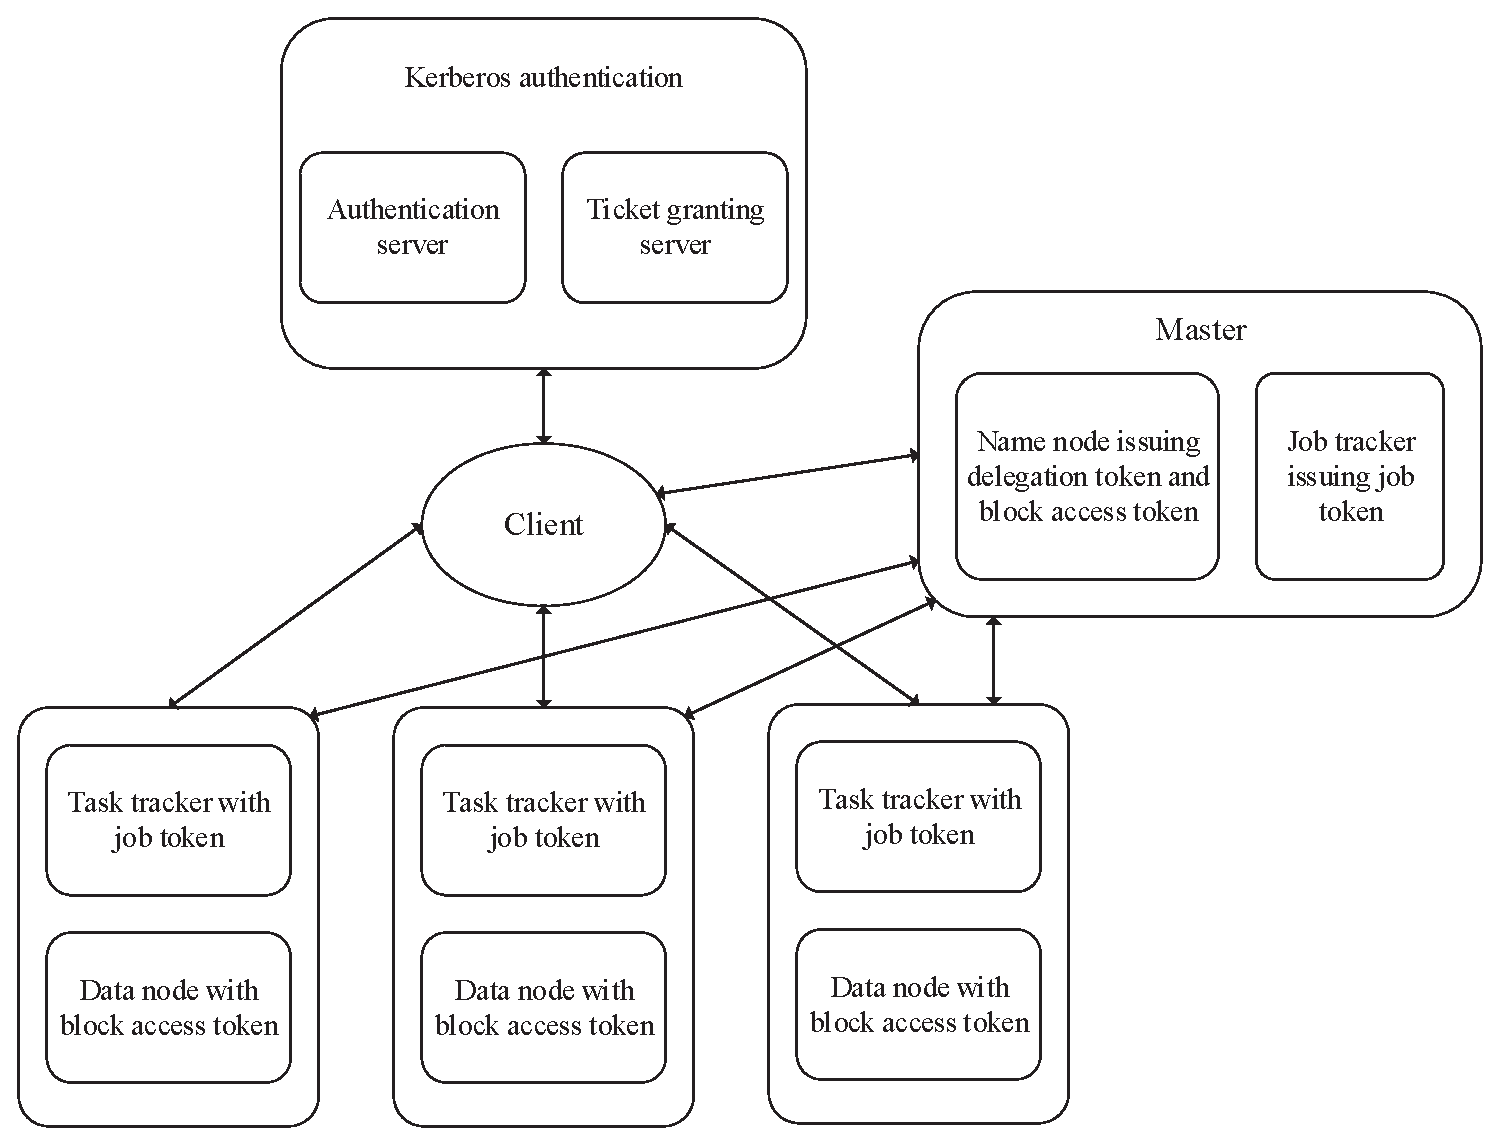
\includegraphics[width=3in]{figs/security_hadoop.eps}
  \caption{Security Framework}
  \label{fig:KerberosOverview}
\end{figure}
In non-secure mode, Hadoop has no authentication, end user accounts which send out communication messages with Hadoop are regarded as Hadoop user accounts by default. For example, different users on different systems with same user name are regarded as same Hadoop user.

In secure mode, Hadoop applies authentication, data confidentiality, and delegation tokens. Kerberos are required for Hadoop authentication in secure mode. Each Hadoop user and service are treated as Kerberos principals, and their permissions are defined in configuration files. To protect transferred data in Hadoop, data encryption are used for Hadoop block data transfer, Hadoop RPC and HTTP communication. The overall architecture of security mechanism is shown in Figure \ref{fig:KerberosOverview}.

As seen in Figure \ref{fig:KerberosOverview}, the Kerberos authentication module has the authentication server and the ticket granting server. Tokens are used to control access to the jobs and data blocks inside HDFS.There exists three types of tokens for HDFS access: 1) delegation token which identifies a user to a particular HDFS service and addresses the problem of propagating authentication performed at job submission time to when the job is later executed; 2) block access token which gives a read or write permission to a HDFS block since the DataNodes do not have any access control list (ACL) mechanism to handle block access; and 3) job token which identifies a map reduce task its jobs.

Hadoop clients use Remote Procedure Call(RPC) which is a Hadoop’s library to access most Hadoop services. In insecure versions of Hadoop, the users login name is determined from the client OS and sent across as part of the connection set-up. For authenticated clusters, all RPC’s connect using Simple Authentication and Secure Layer(SASL). Data Transfer Protocol is used when reading or writing data to HDFS, by clients.

\subsection{Compromised nodes}
Compromised nodes are common in cloud system which means an attacker who has compromised just one node could introduce arbitrary errors into computations, so that the integrity of MapReduce job results could be compromised as well.

This problem is described in Hatman~\cite{khan2012hatman}. Data and computation integrity and security are major concerns for users of cloud computing facilities. Many production-level clouds optimistically assume that all cloud nodes are equally trustworthy when dispatching jobs; jobs are dispatched based on node load, not reputation. This increases their vulnerability to attack, since compromising even one node suffices to corrupt the integrity of many distributed computations. Hatman is the first full-scale, data-centric, reputation-based trust management system for Hadoop clouds. Hatman dynamically assesses node integrity by comparing job replica outputs for consistency.

Since containers provide isolated environment, it could at some extent prevent malicious user on the compromised nodes to tamper MapReduce job results. 
